\LectureAnswerSection\subsection*{两级提示}
\phantomsection\label{hint:at3:drill:1}
\LectureHint{at3:drill:1}{所有速度统一除以内圆速度。}{第二次速度差在外圆交接点计算。}
\phantomsection\label{hint:at3:drill:2}
\LectureHint{at3:drill:2}{在远点比较初速度与当地圆速。}{势能不变，检查动能差中的交叉项。}
\phantomsection\label{hint:at3:drill:3}
\LectureHint{at3:drill:3}{领先角随等待减小。}{加入一整周，选择第一次非负解。}
\phantomsection\label{hint:at3:drill:4}
\LectureHint{at3:drill:4}{脉冲前后位置不变。}{考察到达时圆轨道所需的完整速度状态。}
\phantomsection\label{hint:at3:drill:5}
\LectureHint{at3:drill:5}{先写精确能量差，再按同一小参数展开。}{火箭质量比的近似另需速度增量小于喷速。}
\phantomsection\label{hint:at3:drill:6}
\LectureHint{at3:drill:6}{固定发射速度，反解达到目标所需的最低速度条件。}{检验小范围极限是否回到平地抛射。}
\phantomsection\label{hint:at3:drill:7}
\LectureHint{at3:drill:7}{展开点火前后动能，保留交叉项。}{能量收益相同或不同，都不能单独确定最终轨道。}
\phantomsection\label{hint:at3:drill:8}
\LectureHint{at3:drill:8}{每个脉冲分别比较该点的前后速度。}{速度增量的极限和转移时间的极限一起讨论。}
\phantomsection\label{hint:at3:drill:9}
\LectureHint{at3:drill:9}{短时位移除以轨道半径，形成无量纲比值。}{引力冲量与推力产生的速度增量分别比较。}
\Needspace{8\baselineskip}\subsection*{详解}
\begin{drillsolution}{at3:drill:1}
图\ref{fig:at3:drill:1:s} 令 $v_1=\sqrt{\mu/r_1}$，外圆速度 $v_2=v_1/\sqrt q$。转移近端速度由 $a_t=(1+q)r_1/2$ 得 $v_{t1}=v_1\sqrt{2q/(1+q)}$；远端由角动量守恒得 $v_{t2}=v_1\sqrt{2/[q(1+q)]}$。
\typeout{ASTROFIG:fig:at3:drill:1:p}\fig{fig:at3:drill:1:p}{解答过程：一般双切转移的速度增量}{\begin{tikzpicture}[scale=.85]
\draw[guide](0,0)circle(1.5);\draw[guide](0,0)circle(3);\draw[world](-0.75,0)ellipse(2.25 and 2.1213203435596424);\fill(0,0)circle(2pt)node[below]{$F$};\fill(1.5,0)circle(2pt)node[right]{$A$};\fill(-3,0)circle(2pt)node[left]{$B$};\node at(-.7,1.1){$\Delta v_\Sigma=\Delta v_1+\Delta v_2$};
\end{tikzpicture}}

图\ref{fig:at3:drill:1:p} 两次均为顺行，故
\[\frac{\Delta v_\Sigma}{v_1}=\sqrt{\frac{2q}{1+q}}-1+\frac1{\sqrt q}\left(1-\sqrt{\frac2{1+q}}\right).\]
当 $q\to1$，两项分别趋零。若 $q=1+\epsilon$，各次增量最低阶均为 $v_1\epsilon/4$，总和约 $v_1\epsilon/2$。这个小量检查也能发现漏掉第二次圆化造成的约一半误差。\end{drillsolution}
\begin{drillsolution}{at3:drill:2}
图\ref{fig:at3:drill:2:s} 远点初速 $v_a=\sqrt{2\mu r_p/[r_a(r_p+r_a)]}$，圆化速率为 $v_c=\sqrt{\mu/r_a}$。因此 $\Delta v=v_c-v_a>0$。
\typeout{ASTROFIG:fig:at3:drill:2:p}\fig{fig:at3:drill:2:p}{解答过程：远地点圆化的额外能量}{\begin{tikzpicture}[scale=.85]
\draw[world](-1.5,0)ellipse(3 and 2.598076);\fill(0,0)circle(2pt)node[below right]{$F$};\fill(1.5,0)circle(1.5pt)node[right]{$P$};\fill(-4.5,0)circle(1.5pt)node[left]{$A$};\draw[guide](-4.5,0)--(1.5,0);\node[below]at(-1.5,0){$O$};\node at(-1.5,1){$\Delta\varepsilon=v_a\Delta v+(\Delta v)^2/2$};
\end{tikzpicture}}

图\ref{fig:at3:drill:2:p} 比较前后能量，
\[\Delta\varepsilon=-\frac\mu{2r_a}+\frac\mu{r_p+r_a}
=\frac{\mu(r_a-r_p)}{2r_a(r_p+r_a)}.\]
同一位置的势能没变，代入两速率之差也有 $\Delta\varepsilon=(v_c^2-v_a^2)/2=v_a\Delta v+(\Delta v)^2/2$。这说明不能仅用 $(\Delta v)^2/2$ 当作点火能量。$r_p=r_a$ 时两种轨道本来相同，所需增量为零。\end{drillsolution}
\begin{drillsolution}{at3:drill:3}
图\ref{fig:at3:drill:3:s} 的相对相位随等待减小，不能由较小的 $\phi_0$ 直接增加到 $\phi_*$。应让它先减一整周，再在同余意义上匹配。
\typeout{ASTROFIG:fig:at3:drill:3:p}\fig{fig:at3:drill:3:p}{解答过程：等待下一次转移窗口}{\begin{tikzpicture}[scale=.85]
\draw[axis](-.2,0)--(4.5,0)node[right]{$t$};\draw[axis](0,-.2)--(0,2.4)node[above]{$\phi$};\draw[world](0,1)--(3,-1.3);\draw[guide](0,-1)--(3,-1);\node at(2,1.5){$\phi_*-2\pi$：下一个窗口};
\end{tikzpicture}}

图\ref{fig:at3:drill:3:p} 写 $\phi_0-(n_1-n_2)t=\phi_*-2\pi$，得到
\[t_w=\frac{2\pi+\phi_0-\phi_*}{n_1-n_2},\qquad T_{\rm syn}=\frac{2\pi}{n_1-n_2}.\]
更一般取分子 $(\phi_0-\phi_*)\bmod2\pi$。如果当前已经恰好匹配，第一次非负等待为零；若要求严格未来，则等一个会合周期。不能把得到的负等待时间直接取绝对值，那会选到错误相位。\end{drillsolution}
\begin{drillsolution}{at3:drill:4}
图\ref{fig:at3:drill:4:s} 瞬时脉冲只改速度，位置仍在半径 $r_1$。目标圆轨道的每一个点都满足半径 $r_2$，因而点火后当场不可能已经处于该圆。
\typeout{ASTROFIG:fig:at3:drill:4:p}\fig{fig:at3:drill:4:p}{解答过程：一次变轨能否直接到另一圆轨道}{\begin{tikzpicture}[scale=.85]
\draw[world](0,0)circle(1.6);\draw[world](0,0)circle(3);\fill(0,0)circle(2pt)node[below]{$O$};\node[below]at(1.4,-.8){$r_1$};\node[below]at(2.8,-1.1){$r_2$};\node at(0,3.8){位置连续，圆化状态须同时匹配};
\end{tikzpicture}}

若新轨道以后到达 $r_2$，其状态必须同时满足 $v_r=0,v_t=\sqrt{\mu/r_2}$ 才是目标圆。按 图\ref{fig:at3:drill:4:p} 的无推力唯一运动，这组状态对应的轨道从始至终就是半径 $r_2$ 的圆，不可能此前经过 $r_1\ne r_2$。故一次瞬时脉冲只能进入交会轨道，不能完成不同半径圆轨道间的最终转移；至少还要有后续推力或其他相互作用。\end{drillsolution}
\begin{drillsolution}{at3:drill:5}
图\ref{fig:at3:drill:5:s} 初末能量差为 $\mu[1/r-1/(r(1+\epsilon))]/2$。用 $(1+\epsilon)^{-1}=1-\epsilon+O(\epsilon^2)$ 得 $\Delta\varepsilon=\mu\epsilon/(2r)+O(\epsilon^2)$。
\typeout{ASTROFIG:fig:at3:drill:5:p}\fig{fig:at3:drill:5:p}{解答过程：小幅升轨的能量与耗油}{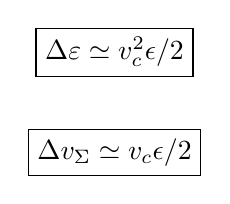
\begin{tikzpicture}[scale=.85]
\node[draw]at(0,1){$\Delta\varepsilon\simeq v_c^2\epsilon/2$};\node[draw]at(0,-.5){$\Delta v_\Sigma\simeq v_c\epsilon/2$};
\end{tikzpicture}}

图\ref{fig:at3:drill:5:p} 的一般双切式在 $q=1+\epsilon$ 下展开，$\Delta v_\Sigma=\tfrac12\sqrt{\mu/r}\,\epsilon+O(\epsilon^2)$。若喷速固定，燃料占初始质量的比例
\[\frac{m_i-m_f}{m_i}=1-\exp(-\Delta v_\Sigma/u)\simeq\frac1{2u}\sqrt{\frac\mu r}\,\epsilon.\]
最后近似还需 $\Delta v_\Sigma\ll u$，它与 $\epsilon\ll1$ 是相关但不同的比较条件。能量增量为一阶，而仅取 $(\Delta v_\Sigma)^2/2$ 是二阶，因而后者漏掉了主要贡献。\end{drillsolution}
\begin{drillsolution}{at3:drill:6}
  图\ref{fig:at3:drill:6:s} 利用达到夹角 $\beta$ 所需的最小速度关系，令 $s=\sin(\beta/2)$、$w=v^2R/\mu<1$，则 $w\ge2s/(1+s)$。
  \typeout{ASTROFIG:fig:at3:drill:6:p}\fig{fig:at3:drill:6:p}{解答过程：给定亚圆速的最大射程角}{\begin{tikzpicture}[scale=.85]
\draw[world](0,0)circle(1.7);\draw[guide](0,0)--(35:1.7)(0,0)--(145:1.7);\node at(0,.8){$\beta_{\max}$};\node at(0,2.5){$\sin(\beta_{\max}/2)=w/(2-w)$};
\end{tikzpicture}}

  按 图\ref{fig:at3:drill:6:p} 单调边界求最大角，$(2-w)s\le w$，所以 $\beta_{\max}=2\arcsin[w/(2-w)]$。达到边界时仰角 $\alpha=\pi/4-\beta_{\max}/4$。若 $w\ll1$，有 $\beta_{\max}\simeq w$，表面弧长约 $R\beta_{\max}=v^2/g$，恢复平地45度最大射程。限定亚圆速使反正弦自变量在零到一之间，也避免把不返回的逃逸初态混入公式。\end{drillsolution}
\begin{drillsolution}{at3:drill:7}
  图\ref{fig:at3:drill:7:s} 两次点火都在各自固定位置，势能瞬间不变。单位质量动能增加分别为 $v_pd+d^2/2$、$v_ad+d^2/2$。
  \typeout{ASTROFIG:fig:at3:drill:7:p}\fig{fig:at3:drill:7:p}{解答过程：近地点与远地点相同增速的能量收益}{\begin{tikzpicture}[scale=.85]
\node[draw]at(0,1){近点：$v_pd+d^2/2$};\node[draw]at(0,-.5){远点：$v_ad+d^2/2$};
\end{tikzpicture}}

  图\ref{fig:at3:drill:7:p} 两者相减得 $(v_p-v_a)d>0$，即近点以同样速度增量获得更多机械能。这并不表示所得目标轨道相同：两处角动量增量分别为 $r_pd,r_ad$，近远点位置和最终形状都不同。若要比较抵达同一目标轨道的燃料，必须把后续修正、圆化以及允许的相位和时间一起算入。\end{drillsolution}
\begin{drillsolution}{at3:drill:8}
  图\ref{fig:at3:drill:8:s} 令初圆速为 $v_0=\sqrt{\mu/r_0}$，用两个椭圆的端点速度逐次求差，得到
  \begin{align*}
  \frac{\Delta v_{\rm bi}}{v_0}={}&\sqrt{\frac{2B}{1+B}}-1
  +\sqrt{\frac{32}{B(B+16)}}-\sqrt{\frac{2}{B(1+B)}}\\
  &+\sqrt{\frac{2B}{16(B+16)}}-\frac14.
  \end{align*}
  \typeout{ASTROFIG:fig:at3:drill:8:p}\fig{fig:at3:drill:8:p}{解答过程：双椭圆转移与无限时间极限}{\begin{tikzpicture}[scale=.85]
\draw[flow](0,0)--(5,0);\node[above]at(0,0){内圆点火};\node[above]at(2.5,0){远点换轨};\node[above]at(5,0){外圆圆化};\node at(2.5,-1){三段速度差相加，时间另作检查};
\end{tikzpicture}}

  图\ref{fig:at3:drill:8:p} 第二项在共同远点顺行，最后一项是到外圆时逆行减速的大小。令 $B\to\infty$，总增量趋于 $(\sqrt2-1)(1+1/4)v_0\simeq0.51777v_0$。双切方案由一般式在 $q=16$ 得约 $0.53624v_0$，因此存在足够大的有限 $B$，三脉冲可以比双切少耗油。可是两段转移半周期都随中间半长轴的 $3/2$ 次方增长，极限所需时间无穷大；这个极限不是有限时间内已经取得的最小值。\end{drillsolution}
\begin{drillsolution}{at3:drill:9}
  图\ref{fig:at3:drill:9:s} 点火时飞船沿轨道移动约 $v_c\tau$，因此几何位置变化相对轨道尺度的比为 $v_c\tau/r=\omega_c\tau$。若此量很小，可将相互作用集中在一个近似固定位置。
  \typeout{ASTROFIG:fig:at3:drill:9:p}\fig{fig:at3:drill:9:p}{解答过程：瞬时脉冲近似的量级检查}{\begin{tikzpicture}[scale=.85]
\node[draw]at(0,1){几何：$v_c\tau/r\ll1$};\node[draw]at(0,-.5){速度：$g_c\tau/\Delta v\ll1$};
\end{tikzpicture}}

  图\ref{fig:at3:drill:9:p} 同时，引力在点火时间内造成速度改变量量级 $g_c\tau$。若还希望把总速度跳变主要视为推力贡献，一个方便的充分条件为 $g_c\tau\ll\Delta v$。因此可以用 $\omega_c\tau\ll1$、$g_c\tau/\Delta v\ll1$ 检查。它们是便于估算的充分条件；更精确的有限点火模型可以同时积分引力和推力，不要求第二项完全忽略。只说“时间短”而不指定与哪个尺度比较，没有明确的误差含义。\end{drillsolution}
